\section{Documentazione del codice}
Il codice che contiene le varie implementazioni della struttura dati è
contenuta nel modulo \texttt{disjoint\_sets}. Questo contiene tre sottomoduli:
\texttt{disjoint\_sets.base}, \texttt{disjoint\_sets.list} e \texttt{disjoint\_sets.tree}.
Il codice utilizzato per rappresentare i grafi e l'operazione di ricerca di componenti
connesse è contenuta nel modulo \texttt{graphs}, mentre il codice usato per il confronto
è nel modulo principale (\texttt{\_\_main\_\_}).

\begin{figure}[!h]
      \centering
      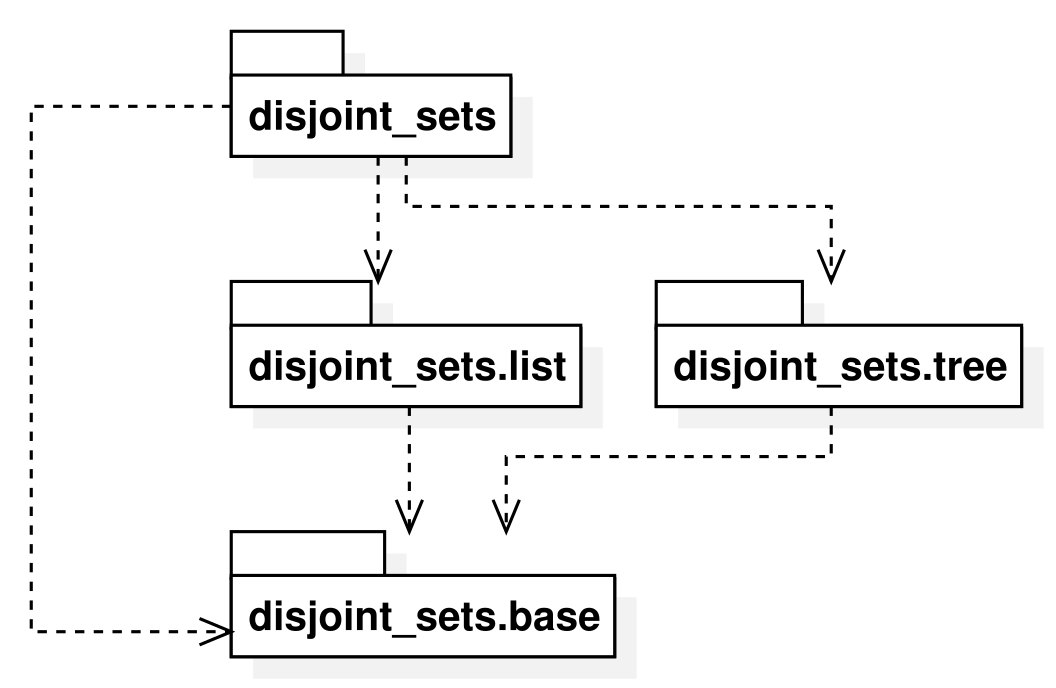
\includegraphics[height=4cm]{diagrams/Package}
      \caption{Diagramma dei moduli utilizzati}
\end{figure}


\subsection{Il modulo \texttt{disjoint\_sets.base}}
Questo modulo contiene le interfacce base per la gestione di
strutture dati per insiemi disgiunti:

\begin{enumerate}
      \item \texttt{Node}: classe per indicare un generico elemento all'interno di un insieme
            disgiunto; contiene un solo attributo \texttt{data} che viene utilizzato per salvare i
            dati relativi all'elemento.
      \item \texttt{DisjointSetsInterface}: interfaccia per le strutture dati che gestiscono
            insiemi disgiunti, contiene i metodi:
            \begin{enumerate}
                  \item \texttt{find\_set(Node) $\rightarrow$ Node}: dato un oggetto \texttt{Node} restituisce il suo rappresentante
                        di tipo \texttt{Node};
                  \item \texttt{make\_set(Any) $\rightarrow$ Node}: data una istanza di un qualsiasi tipo ritorna un oggetto \texttt{Node}
                        con \texttt{data} impostato al valore passato, creando un nuovo insieme disgiunto;
                        \textbf{Nota}: nelle implementazioni contenute nel modulo \texttt{disjoint\_sets} si presuppone che gli elementi
                        inseriti siano tutti diversi tra loro, condizione necessaria per avere insiemi disgiunti, quindi non è presente
                        alcun controllo su tale requisito;
                  \item \texttt{union(Node, Node) $\rightarrow$ Node}: dati 2 oggetti \texttt{Node} esegue l'unione tra i relativi insiemi
                        disgiunti, restituendo il \texttt{Node} nel quale insieme sono stati aggiunti gli elementi dell'insieme
                        dell'altro \texttt{Node} (i.e. restituisce l'oggetto \texttt{Node} il cui insieme non è stato distrutto).
            \end{enumerate}
\end{enumerate}

\subsection{Il modulo \texttt{disjoint\_sets.list}}

\begin{figure}[!b]
      \centering
      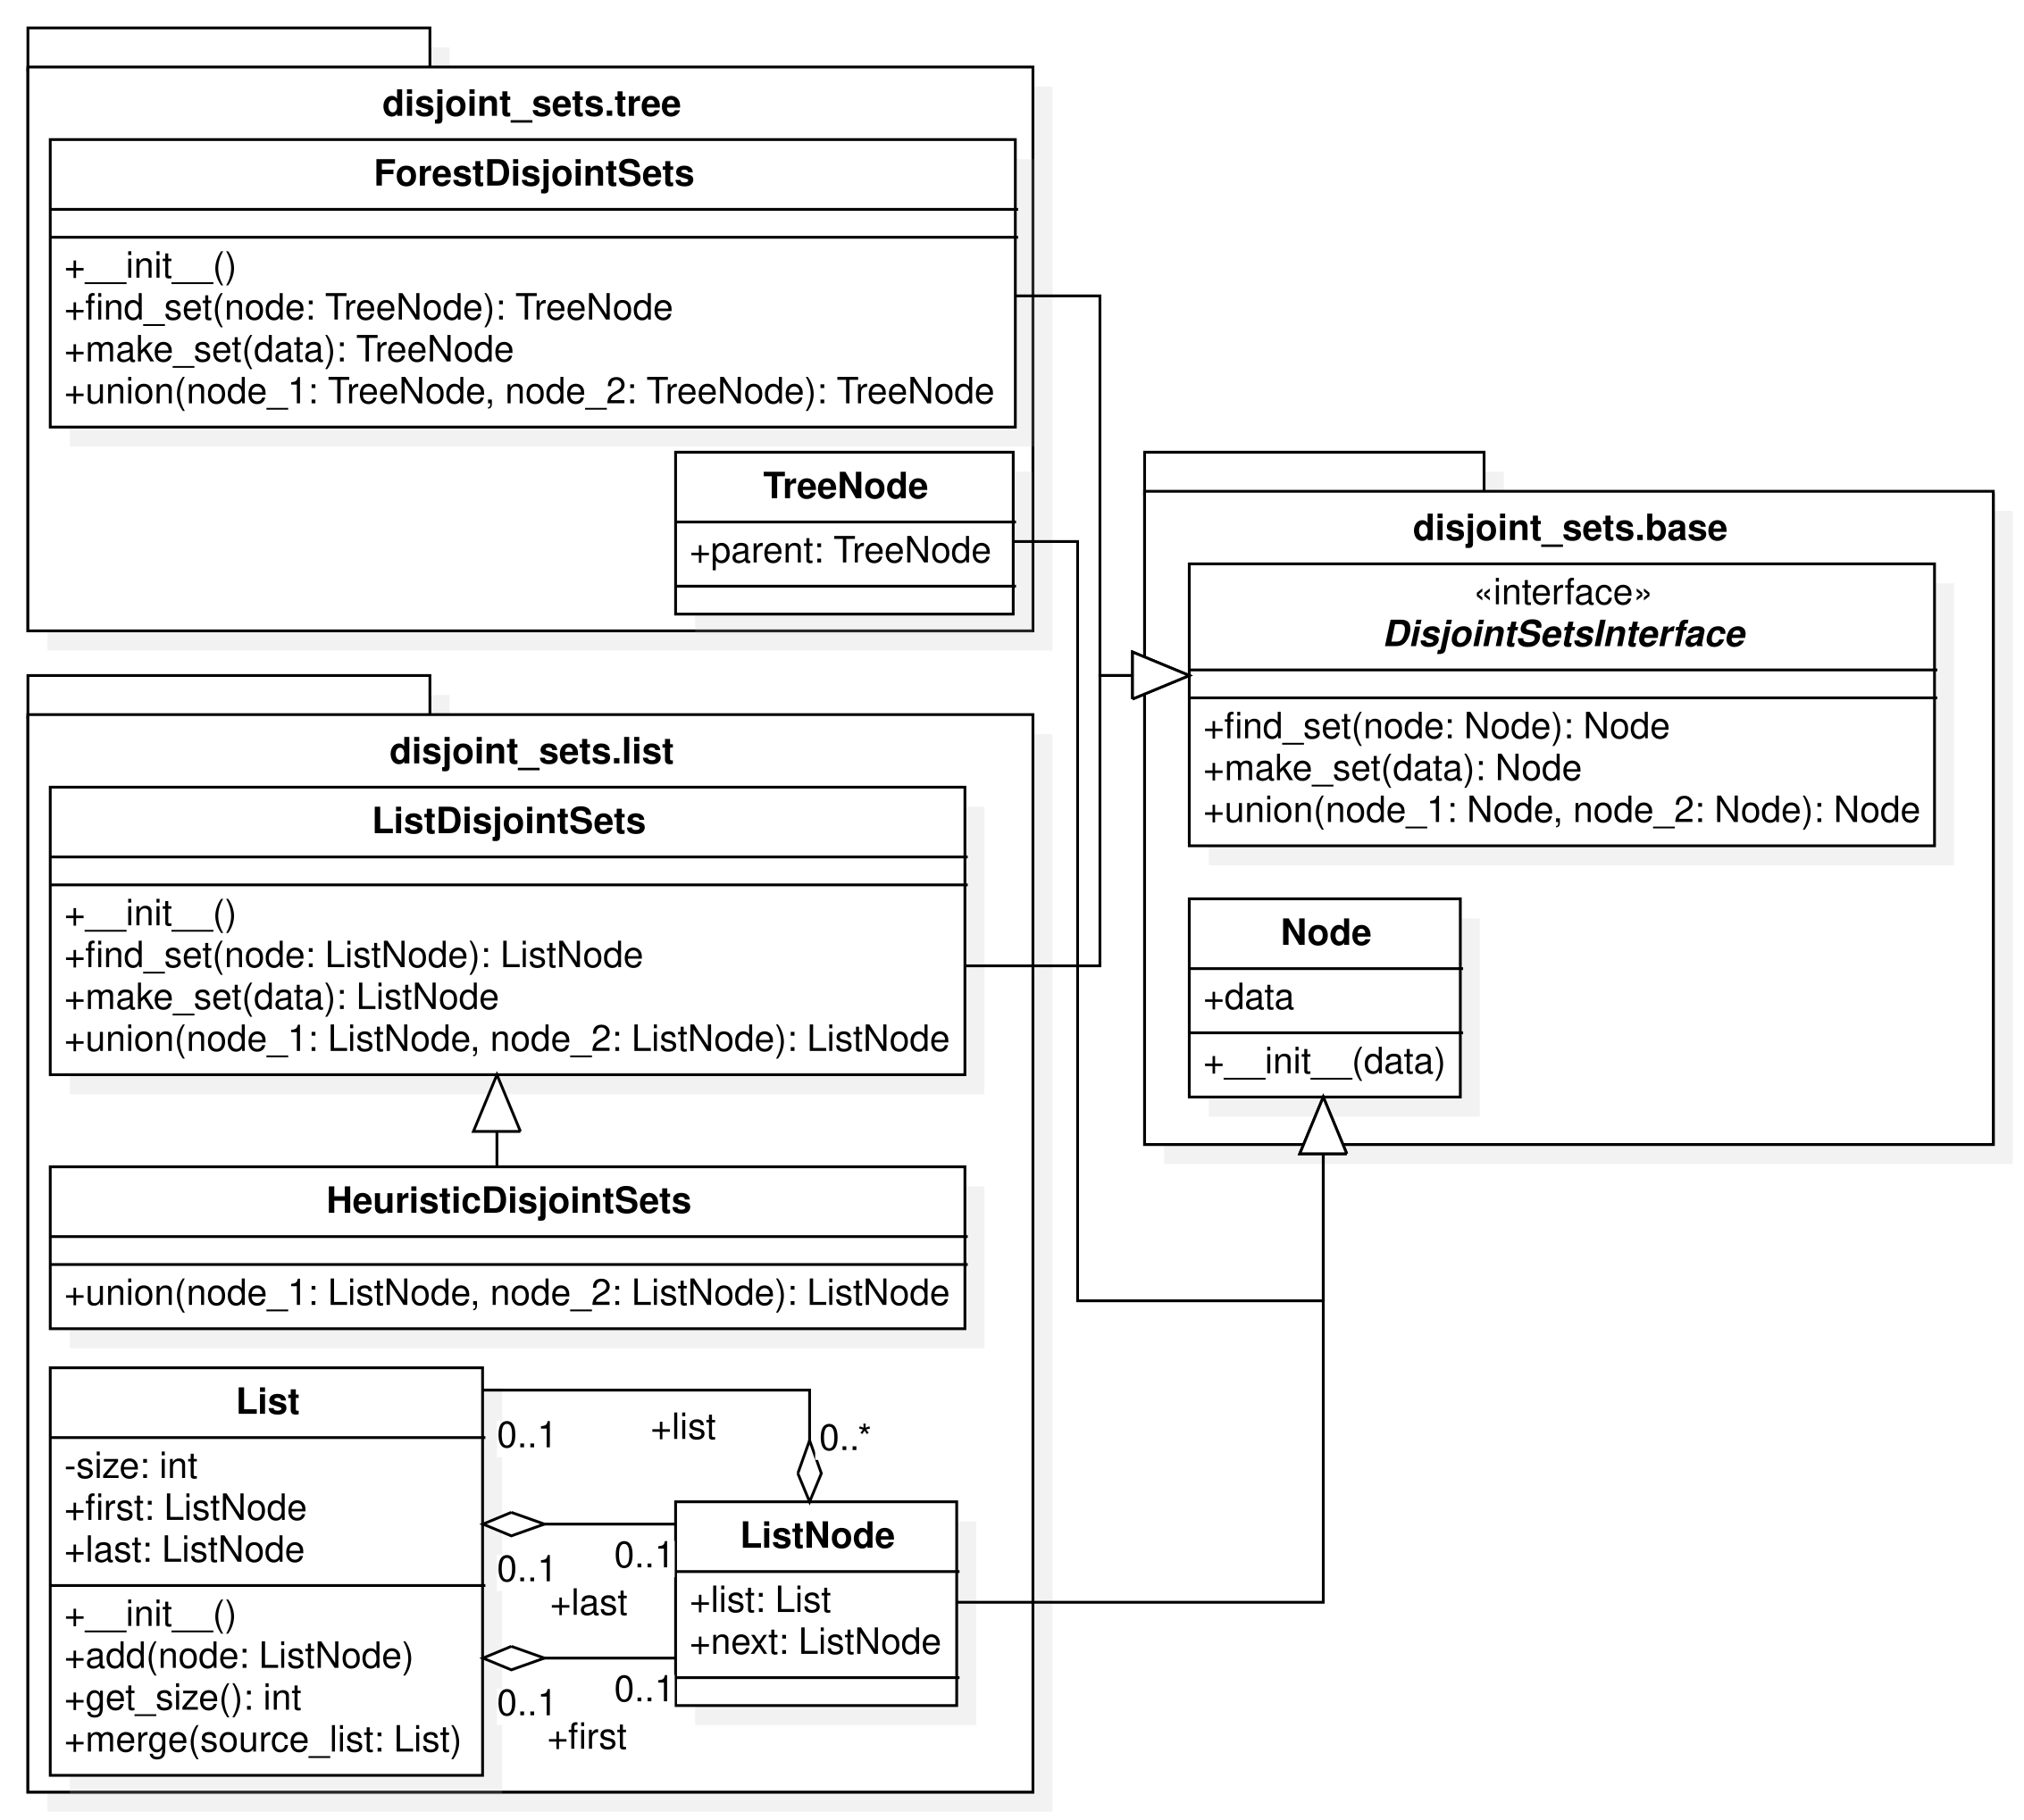
\includegraphics[width=\textwidth]{diagrams/DisjointSets}
      \caption{Diagramma UML del modulo \texttt{disjoint\_sets}}
\end{figure}

Questo modulo contiene le implementazioni delle interfacce tramite liste concatenate con
e senza euristica dell'unione pesata. Sono definite al suo interno le seguenti classi:

\begin{enumerate}
      \item \texttt{ListNode}: eredita \texttt{Node} aggiungendo gli attributi:
            \begin{enumerate}
                  \item \texttt{next $\rightarrow$ Node}: per indicare il successivo elemento (in una lista concatenata)
                  \item \texttt{list $\rightarrow$ List}: anzichè usare un puntatore al rappresentante si usa un puntatore alla lista
                        intera (questo non varia i costi computazionali);
            \end{enumerate}
            \newpage
      \item \texttt{List}: è la struttura dati usata per gestire le liste concatenate e quindi gli insiemi;
            viene inizializzata vuota ed è composta dagli attributi:
            \begin{enumerate}
                  \item \texttt{first $\rightarrow$ ListNode}: rappresenta il primo nodo della lista e quindi il rappresentante;
                  \item \texttt{last $\rightarrow$ ListNode}: rappresenta l'ultimo nodo della lista, fondamentale per gli inserimenti
                        in tempo costante;
                  \item \texttt{\_size $\rightarrow$ int}: attributo privato che rappresenta la dimensione attuale della lista;
            \end{enumerate}
            e dai metodi:
            \begin{enumerate}[resume]
                  \item \texttt{add(ListNode)}: aggiunge alla lista un nodo, incrementando la dimensione della lista;
                  \item \texttt{get\_size() $\rightarrow$ int}: restituisce la dimensione della lista (i.e. elementi
                        contenuti nell'insieme disgiunto);
                  \item \texttt{merge(List)}: inserisce tutti gli elementi di una certa lista nella lista corrente,
                        aggiornando i puntatori verso essa;
            \end{enumerate}
      \item \texttt{ListDisjointSets}: implementazione dell'interfaccia \texttt{DisjointSetsInterface} tramite liste concatenate
            \textbf{senza} euristica dell'unione pesata, tra i metodi
            implementati troviamo alcune particolarità: come detto nella classe \texttt{List} l'operazione di \texttt{find\_set}
            sfrutta il puntatore alla lista per poi ottenere il primo elemento (rappresentante); l'operazione di \texttt{union}
            va a richiamare in modo diretto il metodo \texttt{merge} della lista associata al primo nodo passato come argomento;\newpage
      \item \texttt{HeuristicDisjointSets}: eredita \texttt{ListDisjointSets}, quindi implementa\linebreak \texttt{DisjointSetsInterface}
            per gestire gli insiemi disgiunti tramite liste concatenate \textbf{con} euristica dell'unione pesata: questo implica
            che il metodo \texttt{union} controlli prima le dimensioni delle liste tramite il metodo \texttt{get\_size} e sulla base
            dei esse unisca la lista più corta a quella più lunga.
\end{enumerate}

\subsection{Il modulo \texttt{disjoint\_sets.tree}}
Questo modulo contiene l'implementazione delle interfacce tramite foreste con compressione dei cammini.
A differenza del modulo precedente dove abbiamo \texttt{List} che rappresenta un insieme disgiunto,
in questa implementazione non si ha una classe equivalente (e.g. \texttt{Tree}), e si riduce agli
unici elementi degli alberi. Infatti le classi che lo compongono sono:

\begin{enumerate}
      \item \texttt{TreeNode}: identifica un nodo nell'albero e eredita \texttt{Node} aggiungendo l'attributo \texttt{parent} di tipo \texttt{TreeNode}
            per individuare il padre del nodo; un nodo senza padre diventa automaticamente rappresentante di quell'albero/insieme;
      \item \texttt{ForestDisjointSets}: implementazione dell'interfaccia \texttt{DisjointSetsInterface} per la gestione
            di insiemi disgiunti con foreste di nodi, con compressione dei cammini; tra le operazioni implementate la più degna di nota
            è la \texttt{find\_set} che viene implementata in forma ricorsiva: il caso base si ha quando il nodo passato come argomento
            non ha padre e quindi è il rappresentante, il caso induttivo richiama lo stesso metodo con il padre del nodo e nella fase di
            post-ricorsione si imposta il padre di ogni nodo incontrato con il rappresentante dell'insieme.
\end{enumerate}

\subsection{Il modulo \texttt{graphs}}
Questo modulo definisce le classi per la gestione dei grafi non diretti tramite indici, e fa grande uso delle strutture dati
base messe a disposizione dal linguaggio \textit{Python}:

\begin{figure}[!b]
      \centering
      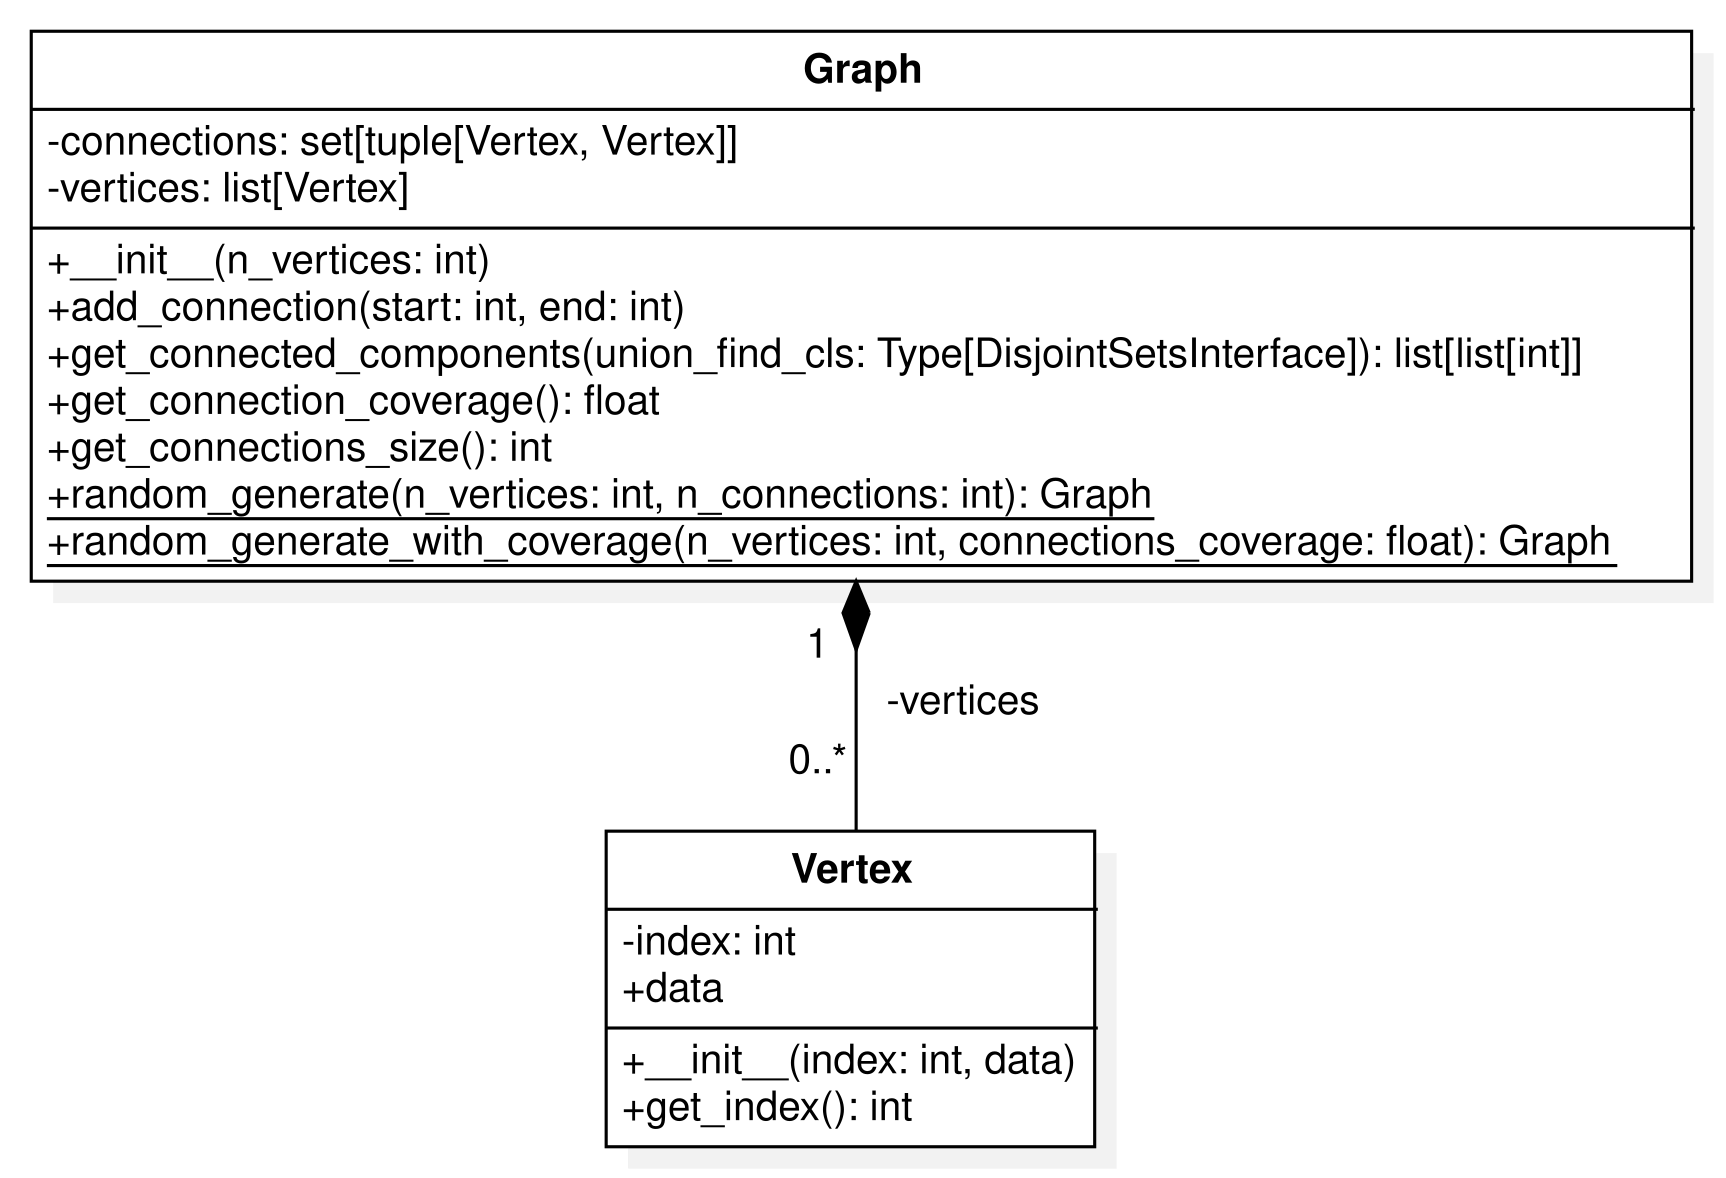
\includegraphics[width=\textwidth]{diagrams/Graph}
      \caption{Diagramma UML del modulo \texttt{graphs}}
\end{figure}

\begin{enumerate}
      \item \texttt{Vertex}: identifica un vertice di un grafo; viene inizializzato con l'indice rispetto
            alla lista di vertici contenuta in nell'oggetto \texttt{Graph} associato, e con il dato associato;
            dato che \texttt{index} è privato, per accedere all'indice del vertice si utilizza il metodo
            \texttt{get\_index() $\rightarrow$ int};\newpage
      \item \texttt{Graph}: è la classe che identifica il grafo non diretto ed è composta dagli attributi:
            \begin{enumerate}
                  \item \texttt{\_vertices $\rightarrow$ list[Vertex]}: attributo privato che salva tutti i
                        vertici del grafo tramite la struttura dati base \texttt{list}; all'istanziazione
                        della classe questa lista viene inizializzata creando un numero di vertici indicato
                        tra i parametri del costruttore;
                  \item \texttt{\_connections $\rightarrow$ set[tuple[Vertex, Vertex]]}: attributo privato usato
                        per salvare le connessioni tra vertici usando le strutture dati base \texttt{tuple} usata
                        per combinare coppie di oggetti in un singolo oggetto e \texttt{set} per gestire un insieme
                        di queste coppie, evitando eventuali duplicati con inserimenti in tempi costanti;
            \end{enumerate}
            e dai metodi:
            \begin{enumerate}[resume]
                  \item \texttt{add\_connection(int, int)}: aggiunge una nuova connessione non diretta tra i vertici
                        usando i relativi indici; gli indici passati vengono riordinati in modo che la sorgente abbia
                        sempre indice minore alla destinazione (anche se in grafi non diretti i termini \textit{sorgente}
                        e \textit{destinazione} non hanno differenza) per ridurre il numero di connessioni salvate nel grafo;
                  \item \texttt{get\_connected\_components(Type[DisjointSetsInterface])\linebreak $\rightarrow$ list[list[int]]}:
                        è il metodo che svolge l'algoritmo \ref{connectedComponentsAlg} utilizzando l'implementazione degli
                        insiemi disgiunti passata come argomento (\texttt{Type[DisjointSetsInterface]} significa che accetta come
                        argomento una \textbf{classe} che implementa \texttt{DisjointSetsInterface}), quindi istanzia la classe
                        passata e la usa nell'algoritmo; oltre a elaborare l'algoritmo il metodo deve ritornarne il risultato
                        della ricerca dato da liste di componenti connesse, ovvero altre liste di indici che rappresentano i vertici,
                        e per fare ciò si fa riferimento al seguente pseudocodice:

                        \begin{algorithm}
                              \caption{Conversione da insiemi disgiunti a liste di liste di vertici}\label{conversion}
                              \begin{algorithmic}[1]
                                    \ENSURE $G(V,E)$ grafo non diretto
                                    \STATE $D\leftarrow$ hash table vuota
                                    \FOR{$v \in G.V$}
                                    \STATE $rep \leftarrow \textsc{Find-Set($v$)}$
                                    \IF{$rep$ \textbf{non} è tra le chiavi di D}
                                    \STATE $D[rep]\leftarrow$ lista vuota
                                    \ENDIF
                                    \STATE aggiungi $v$ a $D[rep]$
                                    \ENDFOR
                                    \RETURN tutti i valori di $D$
                              \end{algorithmic}
                        \end{algorithm}

                        Dobbiamo comunque fare attenzione all'eventuale variazione di costo dell'algoritmo complessivo, infatti abbiamo
                        una variazione del numero di \textsc{Find-Set} eseguite, quindi dato un grafo non diretto $G(V,E)$, si distinguono le implementazioni:
                        \begin{itemize}
                              \item Liste concatenate (\texttt{ListDisjointSets}): in questo caso la \textsc{Find-Set} ha un costo costante
                                    e viene eseguita $|V| = v$ volte, quindi riprendendo \eqref{LLCost} e considerando $n = v$:
                                    \begin{equation}
                                          \Theta(n^2 + v) = \Theta(v^2 + v) = O(v^2)
                                    \end{equation}
                                    quindi non si ha variazione dei costi;
                              \item Liste concatenate con euristica dell'unione pesata\linebreak (\texttt{HeuristicDisjointSets}): anche in
                                    questo caso il costo della \textsc{Find-Set} è costante, e possiamo aggiungere il numero di queste
                                    operazioni a \eqref{WUHValues}:
                                    \begin{equation}
                                          m = n + 3e + n = \Theta(2v + 3e) = \Theta(v + e)
                                    \end{equation}
                                    dimostrando che non vi è alcuna variazione dei costi computazionali;
                              \item Foreste di insiemi disgiunti con compressione dei cammini\linebreak (\texttt{ForestDisjointSets}):
                                    in questo caso il costo della \textsc{Find-Set} non è costante e può richiedere nel caso peggiore
                                    $O(v)$ con $v = |V|$, quindi considerando \eqref{FPCCost}, \eqref{FPCValues} e che il numero di
                                    \textsc{Find-Set} aumenta di $v$ volte:
                                    \begin{equation}
                                          \label{NewFCCCost}
                                          \begin{aligned}
                                                f                                          & = 2 e + v = \Theta(e + v)                                \\
                                                \Theta(n+f\cdot (1+\log_{2+\frac{f}{n}}n)) & = \Theta(v + (e+v) \cdot ( 1+\log_{2+\frac{e+v}{v}}v))   \\
                                                                                           & = O(e\log_{2+\frac{e+v}{v}}v + v\log_{2+\frac{e+v}{v}}v) \\
                                          \end{aligned}
                                    \end{equation}
                                    con un leggera variazione rispetto a \eqref{FPC2Cost}. Ma riconsiderando il costo sulla base del numero di vertici
                                    secondo la copertura lineare \eqref{linearCoverage}:
                                    \begin{equation}
                                          \begin{aligned}
                                                e                  & = \Theta(v)                                           \\
                                                \eqref{NewFCCCost} & = O(v\log_{2+\frac{2v}{v}}v+ v\log_{2+\frac{2v}{v}}v) \\
                                                                   & = O(v\log_4v+ v\log_4v)                               \\
                                                                   & = O(v\log_4v) \simeq O(v\log_3v) = \eqref{linearFPC}
                                          \end{aligned}
                                    \end{equation}
                                    e secondo la copertura quadratica \eqref{quadraticCoverage}:
                                    \begin{equation}
                                          \begin{aligned}
                                                e                  & = \Theta(v^2)                                                       \\
                                                \eqref{NewFCCCost} & = O(v^2\log_{2+\frac{v^2+v}{v}}v+ v\log_{2+\frac{v^2+v}{v}}v)       \\
                                                                   & = O(v^2\log_{3+v}v+ v\log_{3+v}v)                                   \\
                                                                   & = O(v^2\log_{3+v}v) \simeq O(v^2\log_{2+v}v) = \eqref{quadraticFPC}
                                          \end{aligned}
                                    \end{equation}
                                    quindi il costo non varia nemmeno in questo caso;
                        \end{itemize}
                        in generale consideriamo questa operazione come ininfluente nel calcolo dei costi computazionali;
                  \item \texttt{get\_vertices\_size() $\rightarrow$ int}: ritorna il numero di vertici contenuti nel grafo;
                  \item \texttt{get\_connections\_size() $\rightarrow$ int}: ritorna il numero di singole connessioni contenute nel grafo:
                        se si ha una connessione $A \leftrightarrow B$ questa viene contata una sola volta e non come due connessioni distinte
                        $A \rightarrow B$ e $B \rightarrow A$;
                  \item \texttt{get\_connection\_coverage() $\rightarrow$ float}: ritorna la percentuale (compresa tra $[0;1]$) delle connessioni
                        presenti rispetto al numero massimo secondo \eqref{maxedges};
                  \item \texttt{random\_generate(int, \textit{int}) $\rightarrow$ Graph}: metodo statico che permette di generare un'istanza
                        di \texttt{Graph} aggiungendo vertici e connnessioni in maniera casuale; il primo argomento indica il numero di vertici, il secondo
                        il numero di connessioni e quando non è specificato è pari ad un numero casuale compreso tra 0 e il numero massimo di
                        archi possibile secondo \eqref{maxedges}; le connessioni vengono scelte casualmente da un pool generato contenente tutte le possibili
                        connessioni valide utilizzando le librerie \texttt{numpy} e \texttt{itertools};
                  \item \texttt{random\_generate\_with\_poly\_coverage(int, float) $\rightarrow$ Graph}: metodo statico che genera un'istanza
                        di \texttt{Graph} richiamando \texttt{random\_generate}; il primo parametro mantiene lo stesso scopo, il secondo, non più
                        opzionale, rappresenta la copertura polinomiale che viene applicata al grafo secondo \eqref{quadraticCoverage};
                  \item \texttt{random\_generate\_with\_lin\_coverage(int, float) $\rightarrow$ Graph}: metodo statico che si comporta come
                        \texttt{random\_generate\_with\_poly\_coverage}, eccezione per il secondo parametro che rappresenta la copertura lineare
                        che viene applicata al grafo secondo \eqref{linearCoverage};
            \end{enumerate}
\end{enumerate}

\subsection{Il modulo \texttt{\_\_main\_\_}}
Questo modulo rappresenta il file principale del progetto e va ad eseguire i test su diversi grafi utilizzando
le diverse implementazioni per gli insiemi disgiunti.\newline

In prima istanza vengono generati i grafi usati per i test sulla base dei valori di copertura assegnati: per la copertura lineare \texttt{lin}
vengono assegnati i valori \texttt{0.75} e \texttt{1} per evitare eventuali \textit{outliers} senza dover aumentare spropositamente il numero dei vertici
che nei test di copertura lineare assumono i valori $\{1000, 2000, \ldots, 5000\}$; per la copertura quadratica \texttt{poly} vengono assegnati
gli valori \texttt{0.75} e \texttt{1} per avere anche un confronto più corretto tra i due metodi di copertura, ma con numeri di vertici che
assumono i valori $\{100, 200, \ldots, 1000\}$ per evitare lunghi tempi nella generazione dei grafi. Per comprendere meglio la differenza tra copertura
lineare e quadratica e individuare il numero di connesioni effettive, nella tabella \ref{covTable} vengono mostrati i valori di numeri di connessioni
rispetto ai nodi. In totale si hanno $2 \cdot 10 + 2 \cdot 5 = 30$ grafi da testare con le 3 implementazioni degli insiemi disgiunti.\newline

\begin{table}[!h]
      \begin{adjustbox}{center}
            \begin{tabular}{|c|c|c|c|c|c|c|c|}
                  \hline
                  \multicolumn{4}{c|}{Copertura lineare} & \multicolumn{4}{c}{Copertura quadratica}                                                                                                          \\ \hline
                  \multicolumn{2}{|c|}{75\%}             & \multicolumn{2}{c|}{100\%}               & \multicolumn{2}{c|}{75\%} & \multicolumn{2}{c|}{100\%}                                                 \\ \hline
                  Vertici                                & Connessioni                              & Vertici                   & Connessioni                & Vertici & Connessioni & Vertici & Connessioni \\ \hline
                  1000                                   & 750                                      & 1000                      & 1000                       & 100     & 3712        & 100     & 3712        \\ \hline
                  2000                                   & 1500                                     & 2000                      & 2000                       & 200     & 14925       & 200     & 14925       \\ \hline
                  3000                                   & 2250                                     & 3000                      & 3000                       & 300     & 33637       & 300     & 33637       \\ \hline
                  4000                                   & 3000                                     & 4000                      & 4000                       & 400     & 59850       & 400     & 59850       \\ \hline
                  5000                                   & 3750                                     & 5000                      & 5000                       & 500     & 93562       & 500     & 93562       \\ \hline
                                                         &                                          &                           &                            & 600     & 134775      & 600     & 134775      \\ \hline
                                                         &                                          &                           &                            & 700     & 183487      & 700     & 183487      \\ \hline
                                                         &                                          &                           &                            & 800     & 239700      & 800     & 239700      \\ \hline
                                                         &                                          &                           &                            & 900     & 303412      & 900     & 303412      \\ \hline
                                                         &                                          &                           &                            & 1000    & 374625      & 1000    & 374625      \\ \hline
            \end{tabular}
      \end{adjustbox}
      \caption{Numeri di connessioni per nodi basati sui test}
      \label{covTable}
\end{table}

I test vengono quindi fatti passando al metodo \texttt{get\_connected\_components} di ognuno dei grafi le classi che implementano
l'interfaccia \texttt{DisjointSetsInterface} volta per volta e registrando i tempi attraverso la libreria \texttt{time}, sottraendo
il valore finale di \texttt{time.time()} a quello iniziale. Questo processo viene ripetuto per tre volte e alla fine viene calcolata
la mediana dei tempi impiegati per evitare ulteriori \textit{outliers}.\newline

Dopodichè i tempi, arrotondati a 3 cifre dopo la virgola, vengono salvati su un file \texttt{.csv} insieme ai valori di riferimento dei grafi e tramite la libreria \texttt{matplotlib}
vengono visualizzati i grafici dei tempi medi, uno per ogni valore di copertura, dove sull'asse \textit{x} abbiamo i valori dei numeri di vertici mentre
sull'asse \textit{y} i valori dei tempi.


